% Designed Companion Part IV figure
% Intended for \input{...} beside the matching canonical problem.
\begin{figure}[ht]
\centering
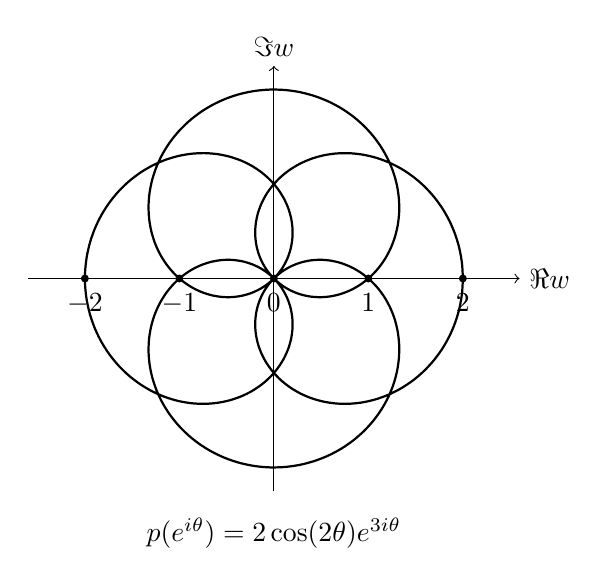
\begin{tikzpicture}[scale=1.2]
  \draw[->] (-2.6,0)--(2.6,0) node[right] {$\Re w$};
  \draw[->] (0,-2.25)--(0,2.25) node[above] {$\Im w$};
  \draw[thick,domain=0:360,samples=240,smooth,variable=\t]
    plot ({2*cos(2*\t)*cos(3*\t)},{2*cos(2*\t)*sin(3*\t)});
  \foreach \x/\lab in {-2/-2,-1/-1,0/0,1/1,2/2} {
    \fill (\x,0) circle (1.2pt);
    \node[below] at (\x,-0.06) {$\lab$};
  }
  \node at (0,-2.7) {$p(e^{i\theta})=2\cos(2\theta)e^{3i\theta}$};
\end{tikzpicture}
\caption{The image $p(\partial\mathbb D)$ is a three-petal curve with real-axis crossings at $-2,-1,0,1,2$. Winding numbers of this curve about a real point $x$ count the roots of $p(z)=x$ inside the unit disk.}
\label{fig:cp-iv-0052-three-petal-image-curve}
\end{figure}
